
%% bare_conf.tex
%% V1.3
%% 2007/01/11
%% by Michael Shell
%% See:
%% http://www.michaelshell.org/
%% for current contact information.
%%
%% This is a skeleton file demonstrating the use of IEEEtran.cls
%% (requires IEEEtran.cls version 1.7 or later) with an IEEE conference paper.
%%
%% Support sites:
%% http://www.michaelshell.org/tex/ieeetran/
%% http://www.ctan.org/tex-archive/macros/latex/contrib/IEEEtran/
%% and
%% http://www.ieee.org/

%%*************************************************************************
%% Legal Notice:
%% This code is offered as-is without any warranty either expressed or
%% implied; without even the implied warranty of MERCHANTABILITY or
%% FITNESS FOR A PARTICULAR PURPOSE! 
%% User assumes all risk.
%% In no event shall IEEE or any contributor to this code be liable for
%% any damages or losses, including, but not limited to, incidental,
%% consequential, or any other damages, resulting from the use or misuse
%% of any information contained here.
%%
%% All comments are the opinions of their respective authors and are not
%% necessarily endorsed by the IEEE.
%%
%% This work is distributed under the LaTeX Project Public License (LPPL)
%% ( http://www.latex-project.org/ ) version 1.3, and may be freely used,
%% distributed and modified. A copy of the LPPL, version 1.3, is included
%% in the base LaTeX documentation of all distributions of LaTeX released
%% 2003/12/01 or later.
%% Retain all contribution notices and credits.
%% ** Modified files should be clearly indicated as such, including  **
%% ** renaming them and changing author support contact information. **
%%
%% File list of work: IEEEtran.cls, IEEEtran_HOWTO.pdf, bare_adv.tex,
%%                    bare_conf.tex, bare_jrnl.tex, bare_jrnl_compsoc.tex
%%*************************************************************************

% *** Authors should verify (and, if needed, correct) their LaTeX system  ***
% *** with the testflow diagnostic prior to trusting their LaTeX platform ***
% *** with production work. IEEE's font choices can trigger bugs that do  ***
% *** not appear when using other class files.                            ***
% The testflow support page is at:
% http://www.michaelshell.org/tex/testflow/



% Note that the a4paper option is mainly intended so that authors in
% countries using A4 can easily print to A4 and see how their papers will
% look in print - the typesetting of the document will not typically be
% affected with changes in paper size (but the bottom and side margins will).
% Use the testflow package mentioned above to verify correct handling of
% both paper sizes by the user's LaTeX system.
%
% Also note that the "draftcls" or "draftclsnofoot", not "draft", option
% should be used if it is desired that the figures are to be displayed in
% draft mode.
%
\documentclass[conference]{IEEEtran}
% Add the compsoc option for Computer Society conferences.
%
% If IEEEtran.cls has not been installed into the LaTeX system files,
% manually specify the path to it like:
% \documentclass[conference]{../sty/IEEEtran}

% Some very useful LaTeX packages include:
% (uncomment the ones you want to load)
\usepackage[utf8]{inputenc}
\usepackage[T1]{fontenc}
%For include figures
\usepackage{graphicx}
\usepackage{epstopdf}
\usepackage{multirow}
\usepackage[brazil]{babel}
\usepackage{hyperref}

% *** MISC UTILITY PACKAGES ***
%
%\usepackage{ifpdf}
% Heiko Oberdiek's ifpdf.sty is very useful if you need conditional
% compilation based on whether the output is pdf or dvi.
% usage:
% \ifpdf
%   % pdf code
% \else
%   % dvi code
% \fi
% The latest version of ifpdf.sty can be obtained from:
% http://www.ctan.org/tex-archive/macros/latex/contrib/oberdiek/
% Also, note that IEEEtran.cls V1.7 and later provides a builtin
% \ifCLASSINFOpdf conditional that works the same way.
% When switching from latex to pdflatex and vice-versa, the compiler may
% have to be run twice to clear warning/error messages.






% *** CITATION PACKAGES ***
%
%\usepackage{cite}
% cite.sty was written by Donald Arseneau
% V1.6 and later of IEEEtran pre-defines the format of the cite.sty package
% \cite{} output to follow that of IEEE. Loading the cite package will
% result in citation numbers being automatically sorted and properly
% "compressed/ranged". e.g., [1], [9], [2], [7], [5], [6] without using
% cite.sty will become [1], [2], [5]--[7], [9] using cite.sty. cite.sty's
% \cite will automatically add leading space, if needed. Use cite.sty's
% noadjust option (cite.sty V3.8 and later) if you want to turn this off.
% cite.sty is already installed on most LaTeX systems. Be sure and use
% version 4.0 (2003-05-27) and later if using hyperref.sty. cite.sty does
% not currently provide for hyperlinked citations.
% The latest version can be obtained at:
% http://www.ctan.org/tex-archive/macros/latex/contrib/cite/
% The documentation is contained in the cite.sty file itself.






% *** GRAPHICS RELATED PACKAGES ***
%
\ifCLASSINFOpdf
  % \usepackage[pdftex]{graphicx}
  % declare the path(s) where your graphic files are
  % \graphicspath{{../pdf/}{../jpeg/}}
  % and their extensions so you won't have to specify these with
  % every instance of \includegraphics
  % \DeclareGraphicsExtensions{.pdf,.jpeg,.png}
\else
  % or other class option (dvipsone, dvipdf, if not using dvips). graphicx
  % will default to the driver specified in the system graphics.cfg if no
  % driver is specified.
  % \usepackage[dvips]{graphicx}
  % declare the path(s) where your graphic files are
  % \graphicspath{{../eps/}}
  % and their extensions so you won't have to specify these with
  % every instance of \includegraphics
  % \DeclareGraphicsExtensions{.eps}
\fi
% graphicx was written by David Carlisle and Sebastian Rahtz. It is
% required if you want graphics, photos, etc. graphicx.sty is already
% installed on most LaTeX systems. The latest version and documentation can
% be obtained at: 
% http://www.ctan.org/tex-archive/macros/latex/required/graphics/
% Another good source of documentation is "Using Imported Graphics in
% LaTeX2e" by Keith Reckdahl which can be found as epslatex.ps or
% epslatex.pdf at: http://www.ctan.org/tex-archive/info/
%
% latex, and pdflatex in dvi mode, support graphics in encapsulated
% postscript (.eps) format. pdflatex in pdf mode supports graphics
% in .pdf, .jpeg, .png and .mps (metapost) formats. Users should ensure
% that all non-photo figures use a vector format (.eps, .pdf, .mps) and
% not a bitmapped formats (.jpeg, .png). IEEE frowns on bitmapped formats
% which can result in "jaggedy"/blurry rendering of lines and letters as
% well as large increases in file sizes.
%
% You can find documentation about the pdfTeX application at:
% http://www.tug.org/applications/pdftex





% *** MATH PACKAGES ***
%
%\usepackage[cmex10]{amsmath}
% A popular package from the American Mathematical Society that provides
% many useful and powerful commands for dealing with mathematics. If using
% it, be sure to load this package with the cmex10 option to ensure that
% only type 1 fonts will utilized at all point sizes. Without this option,
% it is possible that some math symbols, particularly those within
% footnotes, will be rendered in bitmap form which will result in a
% document that can not be IEEE Xplore compliant!
%
% Also, note that the amsmath package sets \interdisplaylinepenalty to 10000
% thus preventing page breaks from occurring within multiline equations. Use:
%\interdisplaylinepenalty=2500
% after loading amsmath to restore such page breaks as IEEEtran.cls normally
% does. amsmath.sty is already installed on most LaTeX systems. The latest
% version and documentation can be obtained at:
% http://www.ctan.org/tex-archive/macros/latex/required/amslatex/math/





% *** SPECIALIZED LIST PACKAGES ***
%
%\usepackage{algorithmic}
% algorithmic.sty was written by Peter Williams and Rogerio Brito.
% This package provides an algorithmic environment fo describing algorithms.
% You can use the algorithmic environment in-text or within a figure
% environment to provide for a floating algorithm. Do NOT use the algorithm
% floating environment provided by algorithm.sty (by the same authors) or
% algorithm2e.sty (by Christophe Fiorio) as IEEE does not use dedicated
% algorithm float types and packages that provide these will not provide
% correct IEEE style captions. The latest version and documentation of
% algorithmic.sty can be obtained at:
% http://www.ctan.org/tex-archive/macros/latex/contrib/algorithms/
% There is also a support site at:
% http://algorithms.berlios.de/index.html
% Also of interest may be the (relatively newer and more customizable)
% algorithmicx.sty package by Szasz Janos:
% http://www.ctan.org/tex-archive/macros/latex/contrib/algorithmicx/




% *** ALIGNMENT PACKAGES ***
%
%\usepackage{array}
% Frank Mittelbach's and David Carlisle's array.sty patches and improves
% the standard LaTeX2e array and tabular environments to provide better
% appearance and additional user controls. As the default LaTeX2e table
% generation code is lacking to the point of almost being broken with
% respect to the quality of the end results, all users are strongly
% advised to use an enhanced (at the very least that provided by array.sty)
% set of table tools. array.sty is already installed on most systems. The
% latest version and documentation can be obtained at:
% http://www.ctan.org/tex-archive/macros/latex/required/tools/


%\usepackage{mdwmath}
%\usepackage{mdwtab}
% Also highly recommended is Mark Wooding's extremely powerful MDW tools,
% especially mdwmath.sty and mdwtab.sty which are used to format equations
% and tables, respectively. The MDWtools set is already installed on most
% LaTeX systems. The lastest version and documentation is available at:
% http://www.ctan.org/tex-archive/macros/latex/contrib/mdwtools/


% IEEEtran contains the IEEEeqnarray family of commands that can be used to
% generate multiline equations as well as matrices, tables, etc., of high
% quality.


%\usepackage{eqparbox}
% Also of notable interest is Scott Pakin's eqparbox package for creating
% (automatically sized) equal width boxes - aka "natural width parboxes".
% Available at:
% http://www.ctan.org/tex-archive/macros/latex/contrib/eqparbox/





% *** SUBFIGURE PACKAGES ***
%\usepackage[tight,footnotesize]{subfigure}
% subfigure.sty was written by Steven Douglas Cochran. This package makes it
% easy to put subfigures in your figures. e.g., "Figure 1a and 1b". For IEEE
% work, it is a good idea to load it with the tight package option to reduce
% the amount of white space around the subfigures. subfigure.sty is already
% installed on most LaTeX systems. The latest version and documentation can
% be obtained at:
% http://www.ctan.org/tex-archive/obsolete/macros/latex/contrib/subfigure/
% subfigure.sty has been superceeded by subfig.sty.



%\usepackage[caption=false]{caption}
%\usepackage[font=footnotesize]{subfig}
% subfig.sty, also written by Steven Douglas Cochran, is the modern
% replacement for subfigure.sty. However, subfig.sty requires and
% automatically loads Axel Sommerfeldt's caption.sty which will override
% IEEEtran.cls handling of captions and this will result in nonIEEE style
% figure/table captions. To prevent this problem, be sure and preload
% caption.sty with its "caption=false" package option. This is will preserve
% IEEEtran.cls handing of captions. Version 1.3 (2005/06/28) and later 
% (recommended due to many improvements over 1.2) of subfig.sty supports
% the caption=false option directly:
%\usepackage[caption=false,font=footnotesize]{subfig}
%
% The latest version and documentation can be obtained at:
% http://www.ctan.org/tex-archive/macros/latex/contrib/subfig/
% The latest version and documentation of caption.sty can be obtained at:
% http://www.ctan.org/tex-archive/macros/latex/contrib/caption/




% *** FLOAT PACKAGES ***
%
%\usepackage{fixltx2e}
% fixltx2e, the successor to the earlier fix2col.sty, was written by
% Frank Mittelbach and David Carlisle. This package corrects a few problems
% in the LaTeX2e kernel, the most notable of which is that in current
% LaTeX2e releases, the ordering of single and double column floats is not
% guaranteed to be preserved. Thus, an unpatched LaTeX2e can allow a
% single column figure to be placed prior to an earlier double column
% figure. The latest version and documentation can be found at:
% http://www.ctan.org/tex-archive/macros/latex/base/



%\usepackage{stfloats}
% stfloats.sty was written by Sigitas Tolusis. This package gives LaTeX2e
% the ability to do double column floats at the bottom of the page as well
% as the top. (e.g., "\begin{figure*}[!b]" is not normally possible in
% LaTeX2e). It also provides a command:
%\fnbelowfloat
% to enable the placement of footnotes below bottom floats (the standard
% LaTeX2e kernel puts them above bottom floats). This is an invasive package
% which rewrites many portions of the LaTeX2e float routines. It may not work
% with other packages that modify the LaTeX2e float routines. The latest
% version and documentation can be obtained at:
% http://www.ctan.org/tex-archive/macros/latex/contrib/sttools/
% Documentation is contained in the stfloats.sty comments as well as in the
% presfull.pdf file. Do not use the stfloats baselinefloat ability as IEEE
% does not allow \baselineskip to stretch. Authors submitting work to the
% IEEE should note that IEEE rarely uses double column equations and
% that authors should try to avoid such use. Do not be tempted to use the
% cuted.sty or midfloat.sty packages (also by Sigitas Tolusis) as IEEE does
% not format its papers in such ways.





% *** PDF, URL AND HYPERLINK PACKAGES ***
%
%\usepackage{url}
% url.sty was written by Donald Arseneau. It provides better support for
% handling and breaking URLs. url.sty is already installed on most LaTeX
% systems. The latest version can be obtained at:
% http://www.ctan.org/tex-archive/macros/latex/contrib/misc/
% Read the url.sty source comments for usage information. Basically,
% \url{my_url_here}.





% *** Do not adjust lengths that control margins, column widths, etc. ***
% *** Do not use packages that alter fonts (such as pslatex).         ***
% There should be no need to do such things with IEEEtran.cls V1.6 and later.
% (Unless specifically asked to do so by the journal or conference you plan
% to submit to, of course. )


% correct bad hyphenation here
\hyphenation{op-tical net-works semi-conduc-tor}


\begin{document}

%
% paper title
% can use linebreaks \\ within to get better formatting as desired
\title{Uma Comparação de Classificadores para Contorno de Imagens de Folhas}


% author names and affiliations
% use a multiple column layout for up to three different
% affiliations

\author{Augusto A. B. Branquinho, Carlos E. S. Sabino, Eduardo C. Campos, Leandro N. Couto\\
Departamento de Ciência da Computação, Universidade Federal de Uberlândia, Uberlândia, MG}
% conference papers do not typically use \thanks and this command
% is locked out in conference mode. If really needed, such as for
% the acknowledgment of grants, issue a \IEEEoverridecommandlockouts
% after \documentclass

% for over three affiliations, or if they all won't fit within the width
% of the page, use this alternative format:
% 
%\author{\IEEEauthorblockN{Michael Shell\IEEEauthorrefmark{1},
%Homer Simpson\IEEEauthorrefmark{2},
%James Kirk\IEEEauthorrefmark{3}, 
%Montgomery Scott\IEEEauthorrefmark{3} and
%Eldon Tyrell\IEEEauthorrefmark{4}}
%\IEEEauthorblockA{\IEEEauthorrefmark{1}School of Electrical and Computer Engineering\\
%Georgia Institute of Technology,
%Atlanta, Georgia 30332--0250\\ Email: see http://www.michaelshell.org/contact.html}
%\IEEEauthorblockA{\IEEEauthorrefmark{2}Twentieth Century Fox, Springfield, USA\\
%Email: homer@thesimpsons.com}
%\IEEEauthorblockA{\IEEEauthorrefmark{3}Starfleet Academy, San Francisco, California 96678-2391\\
%Telephone: (800) 555--1212, Fax: (888) 555--1212}
%\IEEEauthorblockA{\IEEEauthorrefmark{4}Tyrell Inc., 123 Replicant Street, Los Angeles, California 90210--4321}}




% use for special paper notices
%\IEEEspecialpapernotice{(Invited Paper)}




% make the title area
\maketitle


\begin{abstract}
%\boldmath
Este artigo apresenta uma comparação entre diferentes algoritmos de classificação utilizando o {\it Waikato Environment for Knowledge} (WEKA), um software de código aberto com uma coleção de algoritmos de aprendizagem de máquina para tarefas de mineração de dados. O objetivo deste artigo é de investigar a taxa de acertos de diferentes algoritmos de classificação. No processo de classificação foram utilizados os algoritmos \textit{k-Nearest Neighbors} (k-NN), {\it Naive Bayes} (NB), {\it Support Vector Machine} (SVM), Árvore de Decisão J4.8 (J4.8), {\it Random Forest} (RF), {\it Multilayer perceptron} (MLP) e \textit{Linear Discriminant Analysis} (LDA). Na tentativa de melhorar os resultados foram realizados experimentos com algoritmos genéticos (AG) e de seleção de atributos na tentativa de descobrir quais atributos são mais importantes para o de reconhecimento de padrões. Um conjunto de amostras de folhas foi usada para os experimentos. Este conjunto de dados contém informações extraídas dos contornos de 600 imagens de folhas, agrupadas em 30 classes, contendo 20 amostras cada. Cada amostra foi caracterizada por 76 atributos. Desses, os 38 primeiros são baseados em um tipo de medida de imagem, enquanto os 38 seguintes são outro tipo de medição obtida.
\end{abstract}

% IEEEtran.cls defaults to using nonbold math in the Abstract.
% This preserves the distinction between vectors and scalars. However,
% if the conference you are submitting to favors bold math in the abstract,
% then you can use LaTeX's standard command \boldmath at the very start
% of the abstract to achieve this. Many IEEE journals/conferences frown on
% math in the abstract anyway.

% no keywords




% For peer review papers, you can put extra information on the cover
% page as needed:
% \ifCLASSOPTIONpeerreview
% \begin{center} \bfseries EDICS Category: 3-BBND \end{center}
% \fi
%
% For peerreview papers, this IEEEtran command inserts a page break and
% creates the second title. It will be ignored for other modes.
\IEEEpeerreviewmaketitle



\section{Introdução}
% no \IEEEPARstart
O objetivo do nosso trabalho é investigar a taxa de acerto de diferentes algoritmos de classificação. Para isso, os experimentos foram divididos em três partes: a primeira parte utilizou o {\it software} WEKA para a análise de informações extraídas dos contornos de imagens de folhas. A segunda parte utilizou algoritmos genéticos para seleção dos melhores atributos e um ambiente distribuído para execução dos experimentos. Já a terceira parte utilizou o {\it software} MATLAB para realização de experimentos com o método de classificação LDA, cuja implementação não está disponível no WEKA.

Com o intuito de reduzir a dimensionalidade dos dados e melhorar a eficácia dos classificadores, foram realizados experimentos que fazem a seleção ou composição de atributos mais adequados a partir dos originalmente disponíveis. 

Aprendizagem de máquina é um ramo da Inteligência Artificial que lida com a construção e estudo de sistemas que podem aprender a partir dos dados. A extração de informação importante a partir de uma grande pilha de dados e suas correlações é uma grande vantagem dessa área de estudo \cite{IEEEhowto:fauzi}.

A mineração de dados é uma etapa do processo de {\it Knowledge Discovery in Databases} (KDD) que consiste na aplicação de análise de dados e algoritmos de descoberta que, sob as limitações de eficiência computacional aceitáveis, produzem uma enumeração particular de padrões (ou modelos) sobre os dados \cite{IEEEhowto:fayyad}.

O primeiro experimento realizou uma Transformação do Espaço de Atributos utilizando {\it Principal Component Analysis} (PCA) para gerar um novo conjunto de atributos não correlacionados a partir da combinação de projeções dos atributos originais.

O segundo experimento envolveu a utilização de algoritmos genéticos para selecionar quais atributos classificam melhor o conjunto de amostras para cada algoritmo de classificação. 

A Seção 2 descreve a caracterização do problema. Na Seção 3 é feita a fundamentação teórica dos conceitos utilizados no trabalho. A Seção 4 apresenta as ferramentas utilizadas. A seção 5 engloba os experimentos realizados e seus resultados. Na Seção 6 são apresentadas as conclusões do trabalho e alguns possíveis trabalhos futuros. 

% You must have at least 2 lines in the paragraph with the drop letter
% (should never be an issue)

%\hfill January 11, 2007

\section{Caracterização do Problema}

O conjunto de dados contém informações extraídas dos contornos de 600 imagens de folhas, agrupadas em 30 classes contendo 20 amostras cada. Cada amostra é identificada por um total de 76 atributos. Desses, os 38 primeiros são baseados em um tipo de medida de imagem, enquanto que os 38 seguintes são outro tipo de medição obtida.

A Figura \ref{figura:base_folhas} ilustra parte da base de folhas contendo 10 tipos de folhas distintos. Cada tipo de folha representa uma classe. No estudo, foram consideradas 30 classes de folhas.

\begin{figure}[ht]
\centering
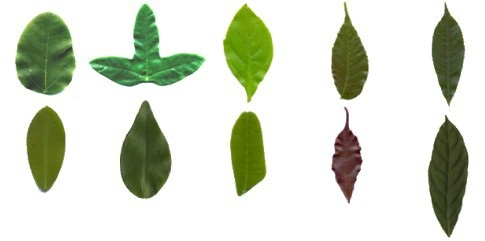
\includegraphics[scale=0.8]{base_folhas.jpg}
\caption{Representação de parte da base de folhas}
\label{figura:base_folhas}
\end{figure}

\section{Fundamentação Teórica}

\subsection{k-Nearest Neighbors}

O algoritmo \textit{k-Nearest Neighbors} (k-NN) é considerado um algoritmo de aprendizagem estatística. Além de ser extremamente simples de implementar, ele é aberto a uma grande variedade de variações. Geralmente é definido em termos da distância Euclidiana \cite{IEEEhowto:fauzi}.

O k-NN é um classificador preguiçoso porque não induz um modelo de categorização de dados de treinamento. O processo de categorização é conseguido através da comparação da nova instância com todas as instâncias do conjunto de dados. Assim, a categoria para a nova instância é selecionada a partir das categorias dos K exemplos mais similares. Em um problema de categorização as entradas são as características e a saída é uma categoria. O k-NN também é conhecido no WEKA como IBK \cite{IEEEhowto:linares}.

\subsection{Naive Bayes}
Os classificadores {\it Naive Bayes} assumem que todos os atributos são independentes e que cada um contribui igualmente para a categorização. A categoria é atribuída a um projeto, combinando a contribuição de cada característica. Esta combinação é atingida estimando as probabilidades {\it a posteriori} de cada categoria utilizando o Teorema de {\it Bayes}. As probabilidades {\it a priori} são estimadas com os dados de treinamento \cite{IEEEhowto:linares}. 

Este tipo de classificador é capaz de lidar com entradas categóricas e problemas de multi-classe. Portanto, em um problema de categorização, as entradas para o classificador são os atributos e a saída é a distribuição de probabilidade do projeto nas categorias \cite{IEEEhowto:linares}.

\subsection{Support Vector Machine}
{\it Support Vector Machine} divide o espaço do problema em dois conjuntos possíveis por encontrar um hiperplano que maximiza a distância com o ponto mais próximo de cada subconjunto. SVM são classificadores binários, mas podem ser utilizados para classificação multi-classe \cite{IEEEhowto:linares}. 

A função que divide o hiperplano é conhecida como função {\it Kernel}. Se os dados são linearmente separáveis, uma função linear {\it Kernel} é usada com o SVM. Nos outros casos, funções não lineares tais como polinômios, funções de base radial (RBF) e sigmóides devem ser utilizadas \cite{IEEEhowto:linares}.	

\subsection{Árvore de Decisão J4.8}
Árvores de decisão são algoritmos que utilizam a estratégia “{\it divide and conquer}” para dividir o espaço do problema em subconjuntos. Uma árvore de decisão é modelada de forma que a raiz e os nós são as perguntas, e os arcos entre os nós são possíveis respostas para as perguntas. As folhas da árvore são categorias \cite{IEEEhowto:linares}.

As árvores de decisão são capazes de lidar com entradas categóricas e os problemas multi-classe. Assim, em um problema de categorização, as entradas para a árvore são os atributos de uma aplicação e a saída é uma categoria \cite{IEEEhowto:linares}.

J4.8 é um algoritmo existente para construção de uma árvore de decisão que permite a manipulação tanto de atributos discretos quanto contínuos. Além disso, permite a manipulação de dados de treinamento com valores de atributos ausentes \cite{IEEEhowto:sandhu}. 
\subsection{Random Forests}
{\it Random Forests} são uma combinação de preditores de árvores de tal modo que cada árvore depende dos valores de um vetor aleatório amostrado de forma independente e com a mesma distribuição para todas as árvores da floresta \cite{IEEEhowto:breiman}. 

{\it Random Forests} são treinadas de forma supervisionada. O treinamento envolve a construção de árvores, bem como a atribuição a cada nó-folha da informação sobre as amostras de treinamento atingindo esse nó-folha (e.g. a distribuição da classe no caso de tarefas de classificação). Em tempo de execução, uma amostra de teste é transmitida a todas as árvores da floresta, e a saída é calculada pela média das distribuições registradas nos nós-folha alcançados \cite{IEEEhowto:lempitsky}.
\subsection{Multilayer Perceptron}
Uma rede {\it Multilayer Perceptron} (MLP) consiste de um conjunto de unidades sensoriais, que constituem a camada de entrada, uma ou mais camada(s) oculta(s) e uma camada de saída. O sinal de entrada propaga-se através da rede para a frente em uma base de camada-a-camada. Uma MLP representa uma generalização da rede {\it Single-layer Perceptron} \cite{IEEEhowto:haykin}.

{\it Multilayer Perceptrons} tem sido aplicadas com sucesso para resolver alguns problemas difíceis e diversos, treinando elas de forma supervisionada com um algoritmo muito popular conhecido como algoritmo de retropropagação do erro ({\it back-propagation}) \cite{IEEEhowto:haykin}.

\subsection{Algoritmos Genéticos}

O algoritmo genético padrão segue o método de reprodução sexuada. Neste algoritmo, a população é composta por um conjunto de indivíduos, de forma que cada indivíduo representa o cromossomo de uma forma de vida \cite{IEEEhowto:prebys}. Os indivíduos correspondem a soluções de um dado problema.

Associado a cada cromossomo é atribuída uma função chamada de \textit{fitness} que determina o quão bom é o indivíduo. Outra função é usada para selecionar os indivíduos da população que iram se reproduzir. Após a seleção de dois indivíduos ocorre o cruzamento ({\it crossover}) dos indivíduos selecionados e eles se dividem novamente. Em seguida, existe uma probabilidade que ocorra a mutação dos novos indivíduos. O processo é repetido durante um certo número de vezes \cite{IEEEhowto:prebys}. Cada repetição corresponde a uma geração. 

\textit{Fitness} é uma medida de "bondade" de um cromossomo, isto é, o quão bem um cromossomo se encaixa no espaço de busca, ou resolve o problema em questão \cite{IEEEhowto:prebys}.

Seleção é o processo de escolha do par de indivíduos para reproduzir \cite{IEEEhowto:prebys}.

{\it Crossover} é um processo de troca de genes entre os dois indivíduos que estão se reproduzindo \cite{IEEEhowto:prebys}.

Mutação é o processo de alteração aleatória dos cromossomos \cite{IEEEhowto:prebys}.

\subsection{Principal Component Analysis}
A Análise dos Componentes Principais (PCA) é uma das técnicas mais bem sucedidas que têm sido utilizada em reconhecimento de imagem e compressão. PCA é um método estatístico cujo propósito é reduzir a grande dimensionalidade do espaço de dados (variáveis observadas) para a menor dimensionalidade instrínseca do espaço de características (variáveis independentes). Este é o caso quando existe uma forte correlação entre as variáveis observadas \cite{IEEEhowto:kim}.

Os trabalhos que PCA pode fazer são previsão, remoção de redundância, extração de características, compressão de dados, entre outros. \cite{IEEEhowto:kim}
\subsection{Linear Discriminant Analysis}
{\it Linear Discriminant Analysis} (LDA) \cite{IEEEhowto:fisher} \cite{IEEEhowto:fukunaga} é um método popular para redução de dimensionalidade linear, que maximiza a dispersão entre as classes e minimiza a dispersão dentro da classe. O LDA tende a dar resultados indesejados se as amostras de alguma classe formam vários agrupamentos distintos, isto é, multimodal \cite{IEEEhowto:fukunaga}. 

Geralmente, o LDA pode se referir a um método de classificação em que primeiramente as amostras de dados são projetadas em uma espaço unidimensional e depois classificadas considerando um {\it thresholding}. A incorporação de um espaço unidimensional utilizada acima é dado como o maximizador do chamado critério de {\it Fisher}. Este critério é frequentemente utilizado para redução de dimensionalidade de um subespaço com dimensão maior que um \cite{IEEEhowto:fukunaga}.
\subsection{Standard Score}
{\it Standard Score} ou {\it Z-Score}, em estatística, é o número de desvios padrão de um dado  acima ou abaixo da média. Um {\it Z-Score} positivo representa um dado acima da média, enquanto que um negativo representa um dado abaixo da média. É uma quantidade desprovida de dimensões obtida subtraindo a média da população de um dado bruto e dividindo o resultado pelo desvio padrão \cite{IEEEhowto:kreyszig}.
\begin{equation}
z=\frac{(x- \mu)}{\sigma} 
\end{equation}
Essa ferramenta é utilizada para diminuir a diferença que escalas podem fazer na classificação de determinados algoritmos.
\section{Ferramentas Utilizadas}
\subsection{WEKA}
O WEKA é um {\it software} de mineração de dados que foi desenvolvido utilizando a linguagem JAVA pela Universidade de {\it Waikato} na Nova Zelândia. Possui uma coleção de algoritmos de aprendizagem de máquina para tarefas de mineração de dados. Ele implementa também algoritmos para pré-processamento de dados, classificação, regressão, {\it clustering} e regras de associação, além de incluir ferramentas de visualização \cite{IEEEhowto:fauzi}. 

O {\it software} encontra-se licenciado ao abrigo da {\it General Public License} (GPL) sendo portanto possível estudar e alterar o respectivo código fonte \cite{IEEEhowto:fauzi}.

O arquivo de dados normalmente utilizado pelo WEKA é o formato de arquivo ARFF ({\it Attribute-Relation File Format}), que consiste de {\it tags} especiais para indicar diferentes elementos no arquivo de dados (e.g. nomes de atributos, tipos de atributos, valores de atributos e os dados) \cite{IEEEhowto:fauzi}.

\subsection{MATLAB} 

O {\it Matrix Laboratory} (MATLAB) é ao mesmo tempo, um ambiente e linguagem de programação para cálculos numéricos com vetores e matrizes. Ele é um produto da empresa {\it The Math Works Inc.} \cite{IEEEhowto:ortega}. 

O MATLAB permite executar tarefas computacionalmente intensivas mais rápido do que com linguagens de programação tradicionais. Ele tem uma ampla variedade de funções úteis para o praticante de algoritmos genéticos \cite{IEEEhowto:furtado}.

\subsection{ECJ}

\textit{Evolutionary Computation Java} (ECJ) consiste em uma biblioteca Java para a execução de algoritmos evolutivos. Ele possui um conjunto de algoritmos já prontos e de fácil extensão. Além disso ele permite o processo de criação e avaliação dos indivíduos de forma distribuída \cite{sean2013}.

Neste trabalho o ECJ foi usado para encontrar melhores atributos usando um AG distribuído.
 
\section{Experimentos}

Os experimentos foram divididos em três partes. Na primeira parte foram realizados experimentos através da interface gráfica do WEKA considerando k-fold igual a 10. A segunda parte utiliza algoritmos genéticos para a seleção dos melhores atributos e um ambiente distribuído para a execução dos experimentos. Por último, foi usado o MATLAB para a execução de um novo conjunto de testes utilizando o algoritmo LDA.

\subsection{Parte 1}

\begin{figure}
\centering
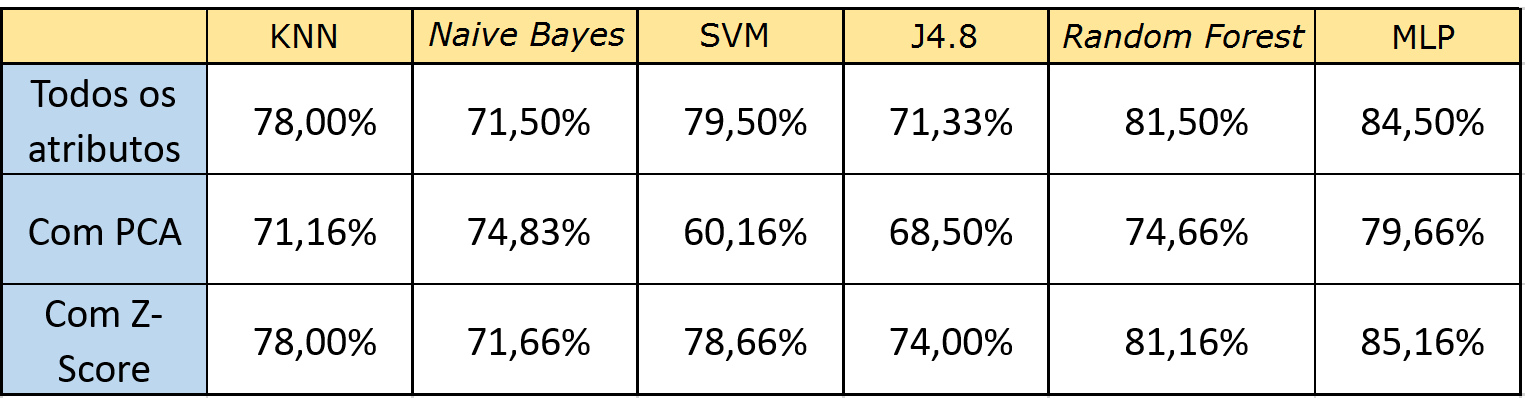
\includegraphics[scale=0.22]{all_atributes.png}
\caption{Taxa de acerto considerando todos os 76 atributos}
\label{figura:all_atributes}
\end{figure}

\begin{figure}
\centering
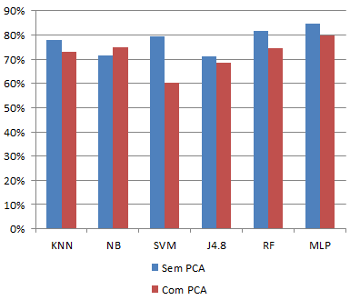
\includegraphics[scale=0.8]{pca76.png}
\caption{Comparação utilizando ou não o PCA nos 76 atributos}
\label{figura:pca76}
\end{figure}

Inicialmente, foram utilizados todos os atributos como entrada para os algoritmos de classificação.
Além disso, foram feitas duas modificações nos atributos na tentativa de melhorar a taxa de classificação correta: normalização dos dados com o algoritmo \textit{Z-Score} e combinação de atributos utilizando o PCA. Estas modificações foram feitas considerando todos os 76 atributos.

A utilização do PCA resultou na geração de seis componentes principais. Todos esses componentes foram considerados no cálculo da taxa de acerto dos algoritmos de classificação, uma vez que ao utilizar menos componentes principais prejudicou o desempenho dos classificadores.

Como podemos observar na Figura \ref{figura:all_atributes}, entre os seis algoritmos utilizados, o que melhor se destacou foi o MLP com o \textit{Z-Score} aplicado, com uma taxa de acerto de 85,16\% das amostras. Ainda na Figura \ref{figura:all_atributes} podemos notar que na utilização do PCA apenas o algoritmo {\it Naive Bayes} se beneficiou, enquanto que todos os outros apresentaram melhores resultados sem nenhuma modificação nos atributos. A taxa de acerto do algoritmo {\it Naive Bayes} utilizando PCA nos 76 atributos foi de 74,83\%. 

A Figura \ref{figura:pca76} ilustra um gráfico comparando a taxa de acerto em \% dos algoritmos de classificação com a utilização do PCA e sem a utilização do PCA. A Fig. 3 ilustra um gráfico comparando a taxa de acerto em \% dos algoritmos de classificação com a utilização do \textit{Z-Score} nos 76 atributos e sem a utilização da normalização.

\begin{figure}
\centering
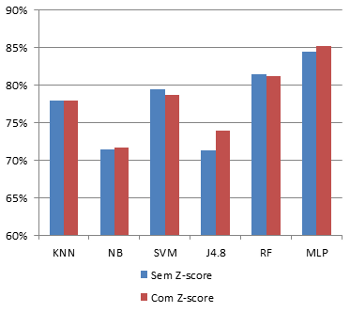
\includegraphics[scale=0.9]{z-score.png}
\caption{Comparação utilizando ou não o Z-Score nos 76 atributos}
\label{figura:z_score}
\end{figure}

Numa segunda abordagem, a base foi dividida em duas partes: 38 primeiros e 38 últimos atributos. Assim como na abordagem inicial, foram utilizados os seis algoritmos definidos anteriormente. Foram feitos dois testes: o primeiro teste aplicou o PCA apenas nos 38 primeiros atributos e o segundo teste aplicou o PCA apenas nos últimos 38 atributos. 
%%% Inicio - Novos comentários sobre experimentos - Eduardo

O resultado do primeiro teste foi a geração de seis componentes principais. A melhor taxa de acerto para os algoritmos foi utilizando todos os seis componentes principais, com exceção do SVM que aumentou sua taxa de acerto de 45,83\% para 47,66\%.

\begin{figure}
\centering
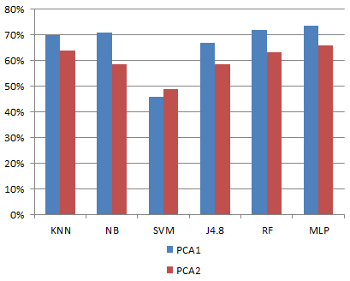
\includegraphics[scale=0.8]{pca38.png}
\caption{Utilizando PCA nos primeiros 38 atributos e nos últimos 38 atributos}
\label{figura_pca38}
\end{figure}

Já no segundo teste, foram gerados apenas três componentes principais. Da mesma forma, a melhor taxa de acerto para os algoritmos foi utilizando todos os três componentes principais. A Fig. 4 representa a comparação entre estes dois testes realizados. O PCA1 refere-se à aplicação do PCA nos primeiros 38 atributos, enquanto que o PCA2 refere-se à aplicação do PCA nos últimos 38 atributos. Logo, podemos concluir que o PCA1 obteve melhores resultados do que o PCA2.

\subsection{Parte 2}

Na segunda parte dos experimentos foi usado um AG para a seleção dos melhores atributos. Para esta tarefa foi usada a ECJ \cite{sean2013}. Esta biblioteca permitiu a execução do algoritmo genético de forma distribuída e paralela. \footnote{O projeto e os \textit{logs} da parte 2 dos experimentos estão disponíveis em: \url{https://code.google.com/p/pgc204/} e \url{http://wpattern.com/blog/post/2013/07/08/ECJ-e-WEKA-(Reconhecimento-de-Padroes).aspx}}

\begin{figure*}
  \centering
  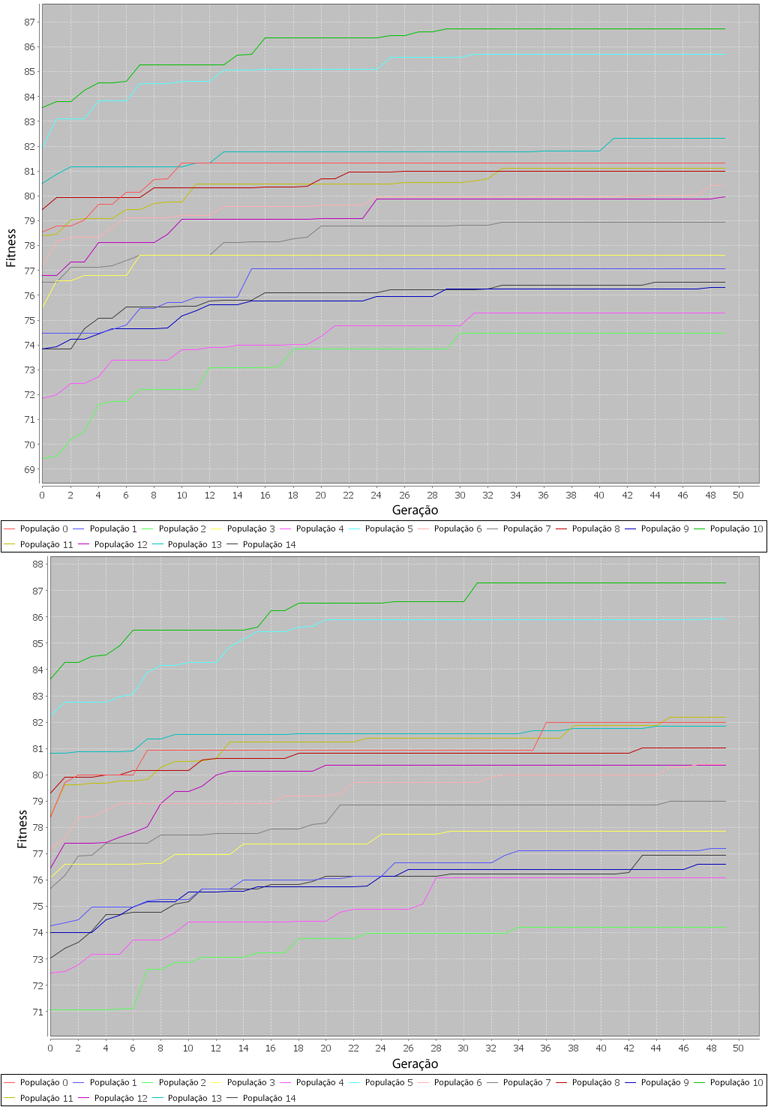
\includegraphics[scale=0.55]{grupo_1_e_grupo_2.png}
  \caption{Gráficos com os percentuais de acerto durante as gerações do AG para os experimentos do grupo 1 e grupo 2, respectivamente.}
  \label{figura:grupo_1_e_grupo_2}
\end{figure*}

O indivíduo foi representado por um cromossomo de 76 genes. Cada gene guarda um valor booleano que determina a presença ou ausência do atributo usado no cálculo do \textit{fitness}. O primeiro gene está associado ao primeiro atributo, o segundo gene ao segundo atributo e assim por diante até o último gene/atributo. A Figura \ref{figura:individuo_do_ag} mostra um exemplo resumido de um indivíduo.

\begin{figure}
  \centering
  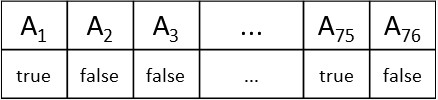
\includegraphics[scale=0.4]{individuo.jpg}
  \caption{Exemplo de um indivíduo usado no AG.}
  \label{figura:individuo_do_ag}
\end{figure}

Foram criadas 30 populações com 50 indivíduos cada. Estas populações foram separadas em dois grupos de 15 populações. No primeiro grupo foi usada a base de dados sem normalização e no outro os dados foram normalizados com o \textit{Z-Score}. Para cada população está associado um algoritmo de reconhecimento de padrões e um conjunto de parâmetros. A Tabela \ref{tabela:populacoes_do_ag} mostra os algoritmos e parâmetros relacionados com cada grupo para suas 15 populações.

\begin{table}[ht]
  \begin{center}
  \caption{Parâmetros usados por cada população do AG.}
  \label{tabela:populacoes_do_ag}
  \begin{tabular}{|c|c|c|}
  \hline
    \textbf{População} & \textbf{Algoritmo} & \textbf{Cross-validation (folds)} \\
  \hline
    0 & k-NN (1) & \multirow{5}{*}{2} \\
  \cline{1-2}
    1 & k-NN (5) & \\
  \cline{1-2}
    2 & k-NN (9) & \\
  \cline{1-2}
    3 & Random Forest & \\
  \cline{1-2}
    4 & Naive Bayes & \\
  \hline
    5 & k-NN (1) & \multirow{5}{*}{5} \\
  \cline{1-2}
    6 & k-NN (5) & \\
  \cline{1-2}
    7 & k-NN (9) & \\
  \cline{1-2}
    8 & Random Forest & \\
  \cline{1-2}
    9 & Naive Bayes & \\
  \hline
    10 & k-NN (1) & \multirow{5}{*}{10} \\
  \cline{1-2}
    11 & k-NN (5) & \\
  \cline{1-2}
    12 & k-NN (9) & \\
  \cline{1-2}
    13 & Random Forest & \\
  \cline{1-2}
    14 & Naive Bayes & \\
  \hline
  \end{tabular}
  \end{center}
\end{table}

Para realizar o cálculo do \textit{fitness} de um indivíduo é executado o algoritmo de reconhecimento de padrões de acordo com a população. A ordem que estão dispostas as amostras durante a execução dos algoritmos influência no percentual de acertos. Sendo assim, antes de qualquer execução a base de dados é reorganizada aleatoriamente e o \textit{fitness} é dado pela média percentual de acertos após 5 execuções.

A população inicial é gerada de forma totalmente aleatória. Para cada população é executado o AG com 50 gerações. Ao final de cada geração são criados 50 novos indivíduos a partir da geração anterior. A seleção dos indivíduos é feita pelo processo de torneio simples. Já o \textit{crossover} ocorre através do sorteio de duas posições (1 até 76) e a respectiva troca de genes entre estas posições. Cada novo indivíduo possui uma chance de 3\% de sofrer mutação, sendo que a mutação apenas altera o valor de um gene que foi escolhido aleatoriamente. Ao final de cada geração os piores indivíduos são eliminados.

Os melhores \textit{fitness's} obtidos após cada geração para cada população do primeiro e segundo grupos são mostrados na Figura \ref{figura:grupo_1_e_grupo_2}.

A melhor indivíduo obtido para o primeiro grupo possui as seguintes características:

\begin{itemize}
  \item Parâmetros da população: k-NN (1) com fold de 10.
  \item Menor \textit{fitness}: $86.33$
  \item \textit{Fitness} médio: $86.73$
  \item Maior \textit{fitness}: $87.16$  
  \item Atributos selecionados: A1, A2, A4, A5, A6, A7, A9, A16, A21, A22, A23, A24, A25, A26, A27, A29, A30, A31, A34, A39, A40, A45, A46, A48, A49, A50, A51, A52, A54, A56, A57, A59, A60, A62, A63, A64, A65, A66, A68, A69, A76.
\end{itemize}

A melhor indivíduo obtido para o segundo grupo possui as seguintes características:

\begin{itemize}
  \item Parâmetros da população: k-NN (1) com fold de 10.
  \item Menor \textit{fitness}: $86.5$
  \item \textit{Fitness} médio: $87.3$
  \item Maior \textit{fitness}: $88.0$  
  \item Atributos selecionados: A1, A2, A4, A5, A7, A8, A9, A10, A11, A16, A17, A18, A20, A21, A22, A23, A25, A26, A27, A28, A29, A31, A32, A33, A34, A37, A39, A40, A46, A47, A49, A50, A51, A53, A54, A55, A57, A58, A60, A61, A63, A65, A66, A67, A69, A71, A73.
\end{itemize}

Conforme é mostrada na Figura \ref{figura:grupo_01_vs_grupo_02}, em geral a normalização dos dados permitiu a obtenção de melhores resultados. Além disso, o algoritmo k-NN com $k = 1$ demonstrou melhores \textit{fitness} que as outras configurações.

\begin{figure}
  \centering
  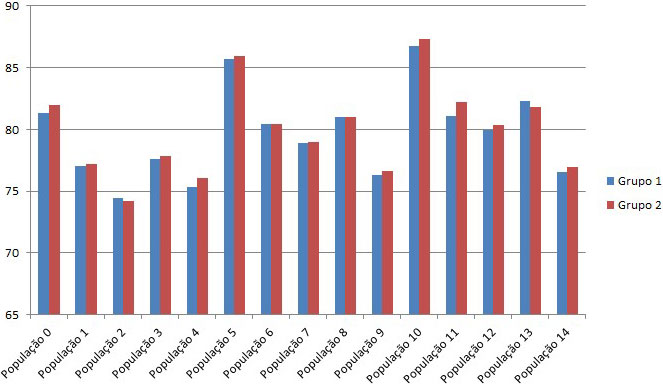
\includegraphics[scale=0.38]{grupo_01_vs_grupo_02.jpg}
  \caption{Comparação dos grupos considerando o \textit{fitness} do melhor indivíduo de cada população após o processo de evolução.}
  \label{figura:grupo_01_vs_grupo_02}
\end{figure}

Apenas neste experimento foram realizados $75000$ execuções de classificação. Como os algoritmos SVM e MLP demandam maior tempo de execução e a quantidade de execuções em geral é grande eles não foram testados. Contudo, este é um dos trabalhos futuros.

\subsection{Parte 3}

Os experimentos com o LDA foram feitos com a implementação do classificador presente no MATLAB considerando k-fold igual a 10. Após a classificação das amostras, foi gerada a matriz de confusão, a partir da qual foram realizadas as análises do método.

Foram realizados quatro testes independentes utilizando o LDA e o PCA:
\begin{enumerate}
  \item Classificação utilizando o LDA nos 76 atributos sem a utilização do PCA;
  \item Utilização do PCA nos 76 atributos e posterior classificação utilizando o LDA;
  \item Utilização do PCA apenas nos 38 primeiros atributos e posterior classificação utilizando o LDA;
  \item Utilização do PCA apenas nos últimos 38 atributos e posterior classificação utilizando o LDA.
\end{enumerate}
 
Os melhores resultados foram obtidos no teste 1, cuja taxa de acerto foi de 88,66\%. No teste 2 foram gerados 6 componentes principais e a taxa de acerto foi de 76,00\%. Já no teste 3 foi obtida uma taxa de acerto de 71,00\%, enquanto que no teste 4, a taxa de acerto foi de 59,67\%.

\section{Conclusão}
Na primeira parte do experimento, o algoritmo de classificação que obteve maior taxa de acerto foi o MLP com {\it Z-score}, que alcançou o valor de 85,16\%. Além disso, podemos concluir que a utilização do PCA nos 76 atributos originais diminuiu a taxa de acerto dos algoritmos de classificação considerados, com exceção do classificador {\it Naive Bayes}, que aumentou sua taxa de acerto atingindo o valor de 74,83\%.

A segunda parte do experimento que envolveu AG em dois grupos de populações mostrou que o algoritmo k-NN configurado com k = 1 e 10 {\it folds} obteve melhores {\it fitness} em ambos os grupos do que as outras configurações. Inclusive o melhor indivíduo do segundo grupo obteve maior {\it fitness} médio (87,3\%) do que o melhor indivíduo do primeiro grupo (86,73\%). O primeiro grupo foi composto por 15 populações de 50 indivíduos cada porém sem a normalização da base de dados, enquanto que o segundo grupo foi composto por 15 populações de 50 indivíduos cada cuja base de dados foi normalizada com {\it Z-Score}. A utilização do AG foi bastante útil na seleção dos melhores atributos.

A terceira parte do experimento que trabalhou com LDA obteve uma taxa de acerto de 88,66\% considerando os 76 atributos originais, ou seja, sem a aplicação do PCA nos atributos. 

Para este tipo de problema, embora o PCA contribuiu para a redução da dimensionalidade do espaço de atributos, sua utilização acarretou uma grande perda de informação nos algoritmos considerados na primeira e terceira partes do experimento. Como exemplo, o SVM foi o mais prejudicado pela utilização do PCA, obtendo uma taxa de acerto de apenas 60,16\%.

Com taxas de classificação abaixo de 90\%, fica evidente que a classificação desse conjunto de dados em particular não configura um problema trivial. A análise do conjunto de dados através do uso de múltiplos métodos de classificação oferece observações importantes em relação à natureza do conjunto de dados.

\subsection*{Trabalhos Futuros}

O AG demonstrou seu poder de encontrar melhores atributos. Contudo, após uma dada quantidade de gerações o \textit{fitness} ficou estagnado. Este cenário ocorre quando o processo de evolução encontrou um máximo local. Para tentar explorar outros máximos locais existe a possibilidade de utilizar uma abordagem de evolução baseado em ilhas \cite{martin1997} ou aumentar a taxa de mutação. Além disso, existe a possibilidade de iniciar populações com diferentes percentuais de presença de atributos, já que isso pode permitir encontrar outros máximos locais. Ainda considerando o AG, existe a necessidade da utilização de outros algoritmos de classificação. Dentre estes algoritmos temos o SVM, LDA e MLP.

% use section* for acknowledgement
%\section*{Agradecimentos}
%The authors would like to thank...


% trigger a \newpage just before the given reference
% number - used to balance the columns on the last page
% adjust value as needed - may need to be readjusted if
% the document is modified later
%\IEEEtriggeratref{8}
% The "triggered" command can be changed if desired:
%\IEEEtriggercmd{\enlargethispage{-5in}}

% references section

% can use a bibliography generated by BibTeX as a .bbl file
% BibTeX documentation can be easily obtained at:
% http://www.ctan.org/tex-archive/biblio/bibtex/contrib/doc/
% The IEEEtran BibTeX style support page is at:
% http://www.michaelshell.org/tex/ieeetran/bibtex/
%\bibliographystyle{IEEEtran}
% argument is your BibTeX string definitions and bibliography database(s)
%\bibliography{IEEEabrv,../bib/paper}
%
% <OR> manually copy in the resultant .bbl file
% set second argument of \begin to the number of references
% (used to reserve space for the reference number labels box)
\begin{thebibliography}{1}

\bibitem{IEEEhowto:fauzi}
M. Fauzi, T. Moh, \emph{Comparison of different classification techniques using WEKA for Breast Cancer}, IFMBE Proceedings, vol. 15, pp. 520-523, 2007.
\bibitem{IEEEhowto:linares}
M. Linares-vásquez, C. Mcmillan, D. Poshyvanyk et al, \emph{On Using Machine Learning to Automatically Classify Software Applications into Domain Categories}, pp. 7-8, 2009.
\bibitem{IEEEhowto:fisher}
R. A. Fisher, \emph{The use of multiple measurements in taxonomic problems. Annals of Eugenics},
7, pp. 179-188, 1936.
\bibitem{IEEEhowto:fukunaga}
K. Fukunaga, \emph{Introduction to statistical pattern recognition}, Boston: Academic Press, Inc. Second edition, 1990. 
\bibitem{IEEEhowto:ortega}
J. Ortega, M. Del, R. Boone et al, \emph{Research issues on K-means Algorithm: An Experimental Trial Using Matlab}, pp. 89-90
\bibitem{IEEEhowto:furtado}
J. Furtado, Z. Cai, L. Xiaobo, \emph{Digital Image Processing: Supervised classification using genetic algorithm in MATLAB Toolbox}, vol. 2, pp.54-55, 2010.
\bibitem{IEEEhowto:sandhu}
L. Sehgal, N. Mohan, P. Sandhu, \emph{Quality Prediction of Function Based Software Using Decision Tree Approach}, International Conference on Computer Engineering and Multimedia Technologies, Bangkok, Thailand, pp. 44-44, 2012.
\bibitem{IEEEhowto:breiman}
L. Breiman, \emph{Random forests}, Statistics Department University of California, Berkley, pp.1-2, 2001.
\bibitem{IEEEhowto:lempitsky}
V. Lempitsky, M. Verhoek, A. Noble et al, \emph{Random Forest Classification for Automatic Delineation of Myocardium in Real-Time 3D Echocardiography}, pp. 449-449, 2009.
\bibitem{IEEEhowto:haykin}
S. Haykin, \emph{Neural Networks: a comprehensive foundation}, Second Edition, pp. 178-179, 1998.
\bibitem{IEEEhowto:kim}
K. Kim, \emph{Face Recognition using Principle Component Analysis}, Department of Computer Science, University of Maryland, USA, pp. 1-1.
\bibitem{IEEEhowto:fayyad}
U. Fayyad, G. Piatetsky-shapiro, P. Smyth, \emph{From Data Mining to Knowledge Discovery in Databases}, pp. 41-41, 1996.
\bibitem{IEEEhowto:prebys}
E. Prebys, \emph{The Genetic Algorithm in Computer Science}, MIT Undergraduate Journal of Mathematics, pp. 166-166.
\bibitem{IEEEhowto:kreyszig}
Kreyszig, E (fourth edition 1979). \emph{Applied Mathmatics}, Wiley Press.
\bibitem{martin1997}
Martin, W. N. and Lienig, J. and Cohoon, J. P. \emph{Island (migration) models: evolutionary algorithms based on punctuated equilibria.} Handbook of Evolutionary Computation. 1997.
\bibitem{sean2013}
Luke, S. \emph{The ECJ Owner’s Manual A User. Manual for the ECJ Evolutionary Computation Library}. Department of Computer Science, George Mason University. May, 2013.
\end{thebibliography}

% that's all folks
\end{document}